\documentclass[11pt,a4paper,oneside]{article}
\usepackage[hangul]{kotex}
\usepackage{olymp}
\usepackage{graphicx}
\usepackage{subcaption}
\usepackage{enumitem}
\usepackage{amsmath}
\usepackage[english]{babel}
\usepackage{amssymb}
\usepackage{import}
\usepackage{multirow}
\usepackage{xcolor}
\usepackage{minted}

% 키파: XeLaTeX 혹은 LuaLaTeX로 컴파일한 뒤 아래 두 줄을 주석해제하면 오류 없이 얼추 비슷한 결과를 얻습니다. 오류 확인을 원할 때 사용하세요.
% \usepackage{fontspec}
% \setmainhangulfont{NanumMyeongjo}

\usepackage{tikz}
\usepackage{pdfpages}


\definecolor{boj}{RGB}{0,118,191}
\definecolor{ucpc-orange}{RGB}{255,153,0}
\definecolor{acgreen}{RGB}{0,159,107}
\definecolor{wared}{RGB}{231,76,60}

\definecolor{acbronze}{RGB}{173,86,0}
\definecolor{acsilver}{RGB}{67,95,122}
\definecolor{acgold}{RGB}{236,154,0}
\definecolor{acplatinum}{RGB}{39,226,164}
\definecolor{acdiamond}{RGB}{0,180,252}
\definecolor{acruby}{RGB}{255,0,98}

%\renewcommand{\baselinestretch}{1.0}

\contest{2024 Soongsil Programming Contest}{SCCC@SoongsilU, Sponsors: FuriosaAI, Hyundai Mobis, Jane Street, Startlink}{May 11th, 2024}

\begin{document}

    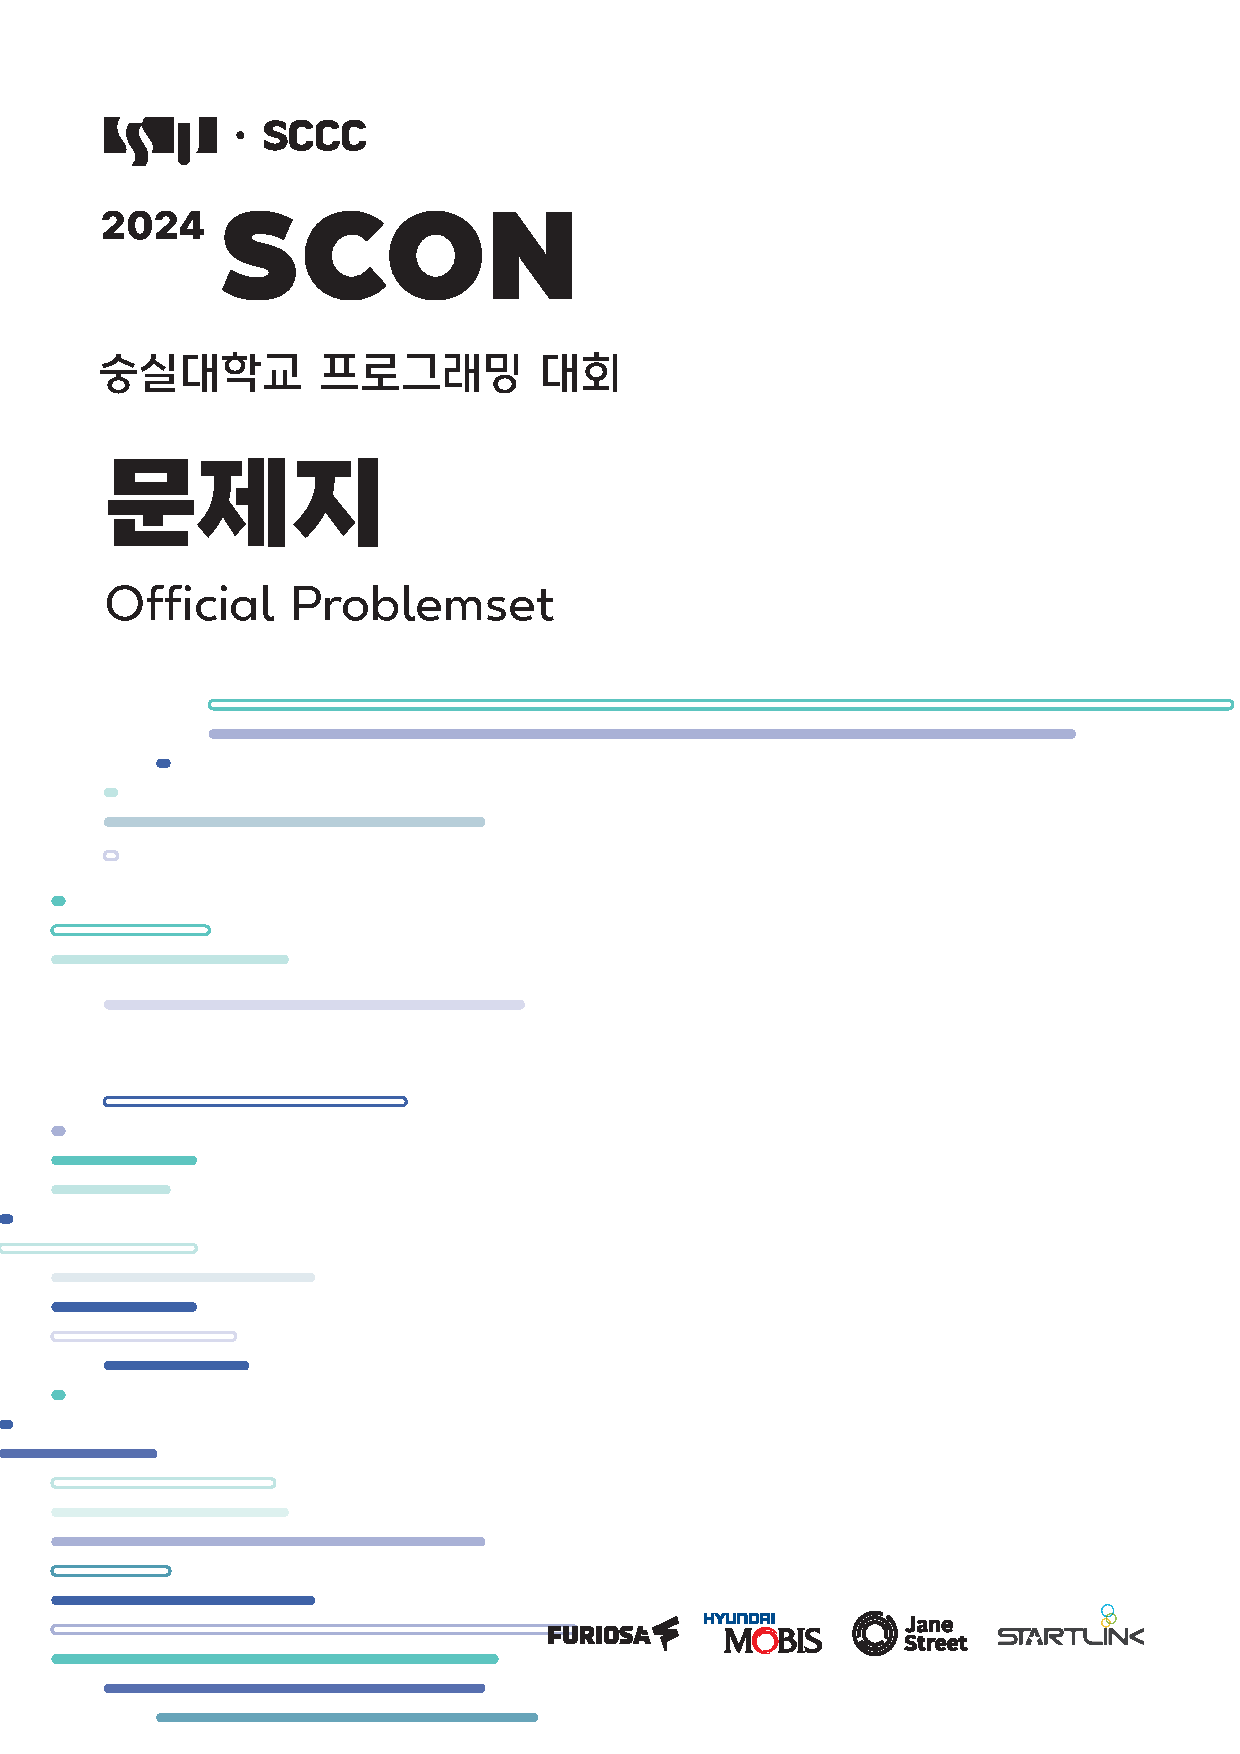
\includepdf[page=1,offset=25mm -38mm]{cover-2024scon.pdf}
%
    \import{./}{language.tex} \pagebreak
    \import{./}{rule.tex} \pagebreak
%
    \begin{center}
    
    \vspace*{15mm}
    {
        \Huge
        \textbf{2024 Soongsil Programming Contest}
        
        \vspace{25mm}
        Problem List
        \vspace{10mm}
    }
    
    \begin{tabular}{|c|l|r|r|r|}
    \hline
    \# & Problem Name & Time limit & Memory limit & Page \\ \hline
        A & 과민성 대장 증후군 & 2 seconds & 1024MiB & \phantom{0}8 -- \phantom{0}8 \\ \hline
        B & 팀명 정하기 2 & 1 second\phantom{s} & 1024MiB & \phantom{0}9 -- 10 \\ \hline
        C & 온데간데없을뿐더러 & 1 second\phantom{s} & 1024MiB & 11 -- 11 \\ \hline
        D & 미로 탈출 & 2 seconds & 1024MiB & 12 -- 12 \\ \hline
        E & 수식 고치기 & 2 seconds & 1024MiB & 13 -- 14 \\ \hline
        F & 피보나치 기념품 & 1 second\phantom{s} & 1024MiB & 15 -- 16 \\ \hline
        G & 시간표 만들기 & 1 second\phantom{s} & 1024MiB & 17 -- 18 \\ \hline
        H & 아이템 2 & 2 seconds & 1024MiB & 19 -- 19 \\ \hline
        I & 불꽃놀이의 아름다움 & 3 seconds & 1024MiB & 20 -- 21 \\ \hline
        J & Traveling SCCC President 2 & 3 seconds & 1024MiB & 22 -- 23 \\ \hline
    \end{tabular}

    \vspace{5mm}
    
    문제지에 있는 문제가 총 10문제가 맞는지 확인하시길 바랍니다.

    문제는 출제진이 생각하는 난이도순으로 정렬되어 있지만, 모든 문제를 읽고 고민하는 것을 권장합니다.

    모든 문제는 C++17, Java 15, PyPy3으로 풀 수 있음을 보장합니다. (단, Python 3는 보장하지 않음)

    I번 문제와 J번 문제는 입출력 양이 매우 많습니다. 2--4페이지에 있는 언어 가이드를 참고하시길 바랍니다.
    
    \end{center}
    	
    \pagebreak

    % \import{sample/}{main.tex} \pagebreak
    \import{2024/irritable-bowel-syndrome/}{main.tex} \pagebreak
    \import{2024/team-name-2/}{main.tex} \pagebreak
    \import{2024/concat/}{main.tex} \pagebreak
    \import{2024/visit-all/}{main.tex} \pagebreak
    \import{2024/modify-expression/}{main.tex} \pagebreak
    \import{2024/fibonacci-partition/}{main.tex} \pagebreak
    \import{2024/create-timetable/}{main.tex} \pagebreak
    \import{2024/fork/}{main.tex} \pagebreak
    \import{2024/beautiful-fireworks/}{main.tex} \pagebreak
    \import{2024/or-path/}{main.tex} \pagebreak
    
\end{document}